\documentclass[12pt]{report}
\usepackage[utf8]{inputenc}
\usepackage[margin=1.2in]{geometry}
\usepackage{graphicx}
\usepackage{float}
\usepackage{subcaption}
\usepackage{amsmath}
\usepackage{amssymb}
\usepackage{ulem}
\usepackage{bm}
\usepackage{framed}
\usepackage{xcolor}
\usepackage{ragged2e}
\usepackage{color}
\usepackage{soul}
\usepackage{cancel}
\graphicspath{ {images/} }
\setlength{\parskip}{1em}
\allowdisplaybreaks


\usepackage{titling}
\newcommand{\subtitle}[1]{%
	\posttitle{%
		\par\end{center}
	\begin{center}\large#1\end{center}
	\vskip0.5em}%
}

\newenvironment{blueframed}[1][blue]
{\def\FrameCommand{\fboxsep=\FrameSep\fcolorbox{#1}{white}}%
\MakeFramed {\advance\hsize-\width \FrameRestore}}
{\endMakeFramed}

\newenvironment{spmatrix}[1]
{\def\mysubscript{#1}\mathop\bgroup\begin{bmatrix}}
{\end{bmatrix}\egroup_{\textstyle\mathstrut\mysubscript}}

\title{Tutorial 9}
\subtitle
{
\textbf{keywords}: variance, error, heteroskedasticity, homoskedasticity, residual plots, Breusch-Pagan test, White test, WLS

\textbf{estimated reading time}: 36 minutes
}
\author{Quang Bui}
\date{September 18, 2018}

\begin{document}

\maketitle

\section*{Question 1}
\noindent EViews workfile: \textit{profits.wf1}

\noindent \textit{(This is a continuation of question 2 in Part A)} The workfile \textit{profits.wf1} includes data on profits and assets of 88 firms (some firms having missing data). The variables in the data set are,
\begin{align*}
profits &- firm's\ profit\ in\ million\ dollars \\
assets &- firm's\ assets\ in\ million\ dollars \\
mno &- a\ dummy\ variable\ which\ equals\ 1\ if\ the\ CEO\ of\ the\ firm\ is\ not\ the\ owner, \\ 
 &0\ otherwise 
\end{align*}
\vspace{-\baselineskip}
%%%%%%%%%% TABLE OBJECT %%%%%%%%%%
\begin{table}[!htbp]
	\centering
	\begin{tabular}{lrrr}
		\multicolumn{1}{c}{}&\multicolumn{1}{r}{PROFITS}&\multicolumn{1}{r}{MNO}&\multicolumn{1}{r}{ASSETS}\\
		\multicolumn{1}{c}{1}&\multicolumn{1}{r}{$66.00$}&\multicolumn{1}{r}{$0.00$}&\multicolumn{1}{r}{$1918.30$}\\
		\multicolumn{1}{c}{2}&\multicolumn{1}{r}{$28.40$}&\multicolumn{1}{r}{$0.00$}&\multicolumn{1}{r}{$789.20$}\\
		\multicolumn{1}{c}{3}&\multicolumn{1}{r}{$18.40$}&\multicolumn{1}{r}{$0.00$}&\multicolumn{1}{r}{$574.30$}\\
		\multicolumn{1}{c}{4}&\multicolumn{1}{r}{$5.80$}&\multicolumn{1}{r}{$0.00$}&\multicolumn{1}{r}{$353.00$}\\
		\multicolumn{1}{c}{5}&\multicolumn{1}{r}{$54.50$}&\multicolumn{1}{r}{$0.00$}&\multicolumn{1}{r}{$568.40$}\\
		\multicolumn{1}{c}{6}&\multicolumn{1}{r}{$3.80$}&\multicolumn{1}{r}{$0.00$}&\multicolumn{1}{r}{$280.00$}\\
		\multicolumn{1}{c}{7}&\multicolumn{1}{r}{$7.40$}&\multicolumn{1}{r}{$0.00$}&\multicolumn{1}{r}{$161.40$}\\
		\multicolumn{1}{c}{8}&\multicolumn{1}{r}{$24.20$}&\multicolumn{1}{r}{$0.00$}&\multicolumn{1}{r}{$274.40$}\\
		\multicolumn{1}{c}{9}&\multicolumn{1}{r}{$4.80$}&\multicolumn{1}{r}{$0.00$}&\multicolumn{1}{r}{$184.60$}\\
		\multicolumn{1}{c}{10}&\multicolumn{1}{r}{$12.80$}&\multicolumn{1}{r}{$0.00$}&\multicolumn{1}{r}{$192.40$}\\
	\end{tabular}
	%\caption{Add your caption here.}
	%\label{tab:}
\end{table}

\vspace{-\baselineskip}
\noindent Our objective is to test the hypothesis that the relationship between profits and assets is the same for owner-managed and non-owner-managed firms. The general model is: $$profits_i = \beta_0 + \delta_0mno_i + \beta_1assets_i + \delta_1 (mno_i \times assets_i) + u_i$$
\noindent \textcolor{red}
{
	(a) Formulate the null hypothesis that the nature of ownership of the firm (i.e. whether the firm is managed by its owner or not) does not affect the relationship between profits and assets in a firm and the alternative that it does.	
}
\begin{align*}
E(profits|mno=0,assets) &= \\
& = 
\end{align*}
\begin{align*}
E(profits|mno=1,assets) &=  \\
& = ts
\end{align*}



\newpage
\noindent \textcolor{red}{(b) Estimate the model using OLS and test whether the errors are homoskedastic using the following tests (in each case, answer the question as if it were a question in the final exam, i.e. write down the null and alternative hypothesis, the test statistics and its distribution under the null, the auxiliary regression you should estimate to compute the test statistic, then compute the test statistic and compare it with the critical value you get from statistical tables):}

\noindent \textcolor{red}{i. Breusch-Pagan test when the alternative hypothesis is $Var(u_i|mno_i , assets_i) = \alpha_0 + \alpha_1 mno_i + \alpha_2 assets_i$}

\noindent \textcolor{red}{ii. White test}

\noindent \textcolor{red}{iii. The special form of the White test that uses the predicted value of $profits$ and its square as predictors of variance.}

\justify
\begin{blueframed}
	\textcolor{blue}{\textbf{Background}}
	\vspace{-\baselineskip}
	\justify
	\textcolor{blue}{\underline{Homoskedasticity and the OLS estimator}}
	
	\noindent \textcolor{blue}
	{
		For a model that is linear in parameters without perfect collinearity, if the assumption for unbiasedness (zero conditional mean) holds, $$E(\textbf{\textit{u}}|\textbf{\textit{X}}) = \textbf{0}$$ the OLS estimator becomes an unbiased linear estimator. If, in addition to the unbiasedness assumption, the errors are serially uncorrelated and homoskedastic, \begin{align*}
		Var(\textbf{\textit{u}}|\textbf{\textit{X}}) &= \sigma^2\textbf{\textit{I}}_n \\
		&=\begin{bmatrix}
		\sigma^2 & 0 & \dots & 0 \\
		0 & \sigma^2 & \vdots & 0 \\
		\vdots & \dots & \ddots & \dots \\
		0 & 0 & \dots & \sigma^2
		\end{bmatrix}
		\end{align*} $$(off\ diagonal\ elements = 0 \implies unserially\ uncorrelated\ errors)$$ $$(diagonal\ elements = \sigma^2 \implies homoskedastic\ errors)$$ then the OLS estimator becomes the \textit{most efficient linear unbiased estimator}. \\ \\ \uline{Consequences of heteroskedastic errors} \begin{itemize}
			\item If all Gauss-Markov assumptions hold, except the assumption of homoskedastic errors, then the OLS estimator is no longer BLUE i.e. the OLS estimator is not the best linear unbiased estimator.
		\end{itemize}  
	}
\end{blueframed}
\begin{blueframed}
	\noindent \textcolor{blue}
	{
		\begin{itemize}
			\item A more several consequence is that the $t$ and $F$ test statistics not longer have a $t$ and $F$ distribution, so the $t$ and $F$ test are no longer valid.
		\end{itemize}
		\uline{Understanding the variance of the error: $Var(\boldsymbol{u}|\boldsymbol{X}) = Var(\boldsymbol{y}|\boldsymbol{X})$} \\ \\ In our model of a firm's $profit$, $$profits_i = \beta_0 + \delta_0mno_i + \beta_1assets_i + \delta_1 mno_i \times assets_i + u_i$$ the error term is homoskedastic if the variance of the error is constant i.e. the variance is fixed across all $i$ (if the error does not vary differently across different $i$ then it is constant regardless of the value of $x$), $$Var(u_i|mno_i,assets_i) = \sigma^2$$ If the error term is heteroskedastic, then the variance of the error is not constant, $$Var(u_i|mno_i,assets_i) \neq \sigma^2$$ 
		Since $\beta_0$, $\beta_1$, $\delta_0$, and $\delta_1$ are constants and $mno_i$ and $assets_i$ are known (we have conditioned on $mno_i$ and $assets_i$),
		\begin{align*}
		Var(profit_i|mno_i,assets_i) &= Var(\beta_0 + \delta_0mno_i + \beta_1assets_i + \delta_1 mno_i \times assets_i \\ &+ u_i|inc_i,nf_i) \\ 
		&= Var(u_i|mno_i,assets_i)
		\end{align*}
		This tells us that if the variance of the dependent variable is not constant, then the variance of the error will not be constant i.e. the error is heteroskedastic.
	}
\end{blueframed}


\noindent \textcolor{red}{Estimate the model using OLS, then save the residuals (the 3 test for heteroskedasticity requires running a regression with the squared residual as the dependent variable).}

\noindent From the Command window:
$$ls\ profit\ c\ mno\ assets\ mno^*assets$$
\begin{figure}[H]
	\centering
	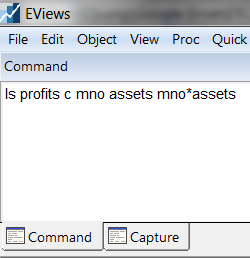
\includegraphics{q1_1}
\end{figure}
\vspace{-\baselineskip}
%%%%%%%%%% TABLE OBJECT %%%%%%%%%%
\begin{table}[!htbp]
	\centering
	\begin{tabular}{lrrrr}
		\multicolumn{3}{l}{Dependent Variable: PROFITS}&\multicolumn{1}{c}{}&\multicolumn{1}{c}{}\\
		\multicolumn{3}{l}{Method: Least Squares}&\multicolumn{1}{c}{}&\multicolumn{1}{c}{}\\
		\multicolumn{3}{l}{Date: 09/15/18   Time: 17:13}&\multicolumn{1}{c}{}&\multicolumn{1}{c}{}\\
		\multicolumn{2}{l}{Sample: 1 88}&\multicolumn{1}{c}{}&\multicolumn{1}{c}{}&\multicolumn{1}{c}{}\\
		\multicolumn{3}{l}{Included observations: 69}&\multicolumn{1}{c}{}&\multicolumn{1}{c}{}\\
		[4.5pt] \hline \\ [-4.5pt]
		\multicolumn{1}{c}{Variable}&\multicolumn{1}{r}{Coefficient}&\multicolumn{1}{r}{Std. Error}&\multicolumn{1}{r}{t-Statistic}&\multicolumn{1}{r}{Prob.}\\
		[4.5pt] \hline \\ [-4.5pt]
		\multicolumn{1}{c}{C}&\multicolumn{1}{r}{$1.561369$}&\multicolumn{1}{r}{$2.780089$}&\multicolumn{1}{r}{$0.561626$}&\multicolumn{1}{r}{$0.5763$}\\
		\multicolumn{1}{c}{MNO}&\multicolumn{1}{r}{$8.231865$}&\multicolumn{1}{r}{$4.087202$}&\multicolumn{1}{r}{$2.014059$}&\multicolumn{1}{r}{$0.0481$}\\
		\multicolumn{1}{c}{ASSETS}&\multicolumn{1}{r}{$0.050647$}&\multicolumn{1}{r}{$0.006196$}&\multicolumn{1}{r}{$8.174306$}&\multicolumn{1}{r}{$0.0000$}\\
		\multicolumn{1}{c}{MNO*ASSETS}&\multicolumn{1}{r}{$-0.052172$}&\multicolumn{1}{r}{$0.009294$}&\multicolumn{1}{r}{$-5.613231$}&\multicolumn{1}{r}{$0.0000$}\\
		[4.5pt] \hline \\ [-4.5pt]
		\multicolumn{1}{l}{R-squared}&\multicolumn{1}{r}{$0.521963$}&\multicolumn{2}{l}{Mean dependent var}&\multicolumn{1}{r}{$12.83188$}\\
		\multicolumn{1}{l}{Adjusted R-squared}&\multicolumn{1}{r}{$0.499900$}&\multicolumn{2}{l}{S.D. dependent var}&\multicolumn{1}{r}{$18.62111$}\\
		\multicolumn{1}{l}{S.E. of regression}&\multicolumn{1}{r}{$13.16843$}&\multicolumn{2}{l}{Akaike info criterion}&\multicolumn{1}{r}{$8.049745$}\\
		\multicolumn{1}{l}{Sum squared resid}&\multicolumn{1}{r}{$11271.50$}&\multicolumn{2}{l}{Schwarz criterion}&\multicolumn{1}{r}{$8.179258$}\\
		\multicolumn{1}{l}{Log likelihood}&\multicolumn{1}{r}{$-273.7162$}&\multicolumn{2}{l}{Hannan-Quinn criter.}&\multicolumn{1}{r}{$8.101127$}\\
		\multicolumn{1}{l}{F-statistic}&\multicolumn{1}{r}{$23.65757$}&\multicolumn{2}{l}{Durbin-Watson stat}&\multicolumn{1}{r}{$2.410291$}\\
		\multicolumn{1}{l}{Prob(F-statistic)}&\multicolumn{1}{r}{$0.000000$}&\multicolumn{1}{c}{}&\multicolumn{1}{c}{}&\multicolumn{1}{c}{}\\
		[4.5pt] \hline \\ [-4.5pt]
	\end{tabular}
	%\caption{Add your caption here.}
	%\label{tab:}
\end{table}


\noindent Save the OLS residuals into a separate series (the series $resid$ contains the residuals from the last estimated model),
$$Proc \to Make\ to\ Residual\ Series \to Name\ for\ resid:uhat \to OK$$
\begin{figure}[H]
	\centering
	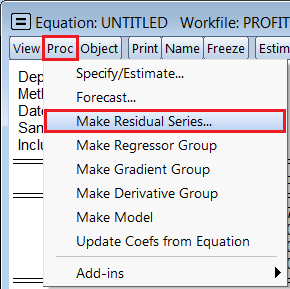
\includegraphics{q1_2}
\end{figure}
\vspace{-\baselineskip}
\begin{figure}[H]
	\centering
	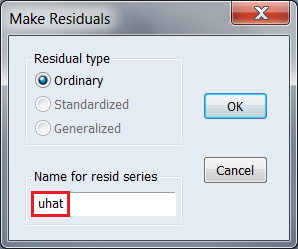
\includegraphics{q1_3}
\end{figure}
\vspace{-\baselineskip}
\begin{figure}[H]
	\centering
	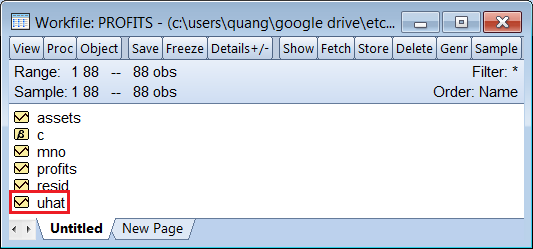
\includegraphics{q1_11}
\end{figure}
\vspace{-\baselineskip}

\newpage
\justify
\begin{blueframed}
	\textcolor{blue}{\textbf{Background}}
	\vspace{-\baselineskip}
	\justify
	\textcolor{blue}{\underline{Breusch-Pagan test for heteroskedasticity}}
	
	\noindent \textcolor{blue}
	{
		\noindent Since $E(u_i|mno_i,assets_i)=0$, 
		\begin{align*}
		Var(u_i|mno_i,assets_i) &= E(u^2_i|mno_i,assets_i) - (E(u_i|mno_i,assets_i))^2 \\
		&= E(u^2_i|mno_i,assets_i)
		\end{align*}
		\noindent we can think about a possible `model' for the $Var(u_i|mno_i,assets_i)$ i.e. one that contains variables to help explain $Var(u_i|mno_i,assets_i)$. \\ \\ By considering a model of the squared error term from our model of firm's profits, 
		\begin{align*}
		u^2_i &= \delta_0 + \delta_1z_{i1} + \delta_2z_{i2} + \dots + \delta_qz_{iq} + v_i \\
		&= E(u^2_i|z_{i1},z_{i2},\dots,z_{iq}) + v_i \\ 
		&= Var(u_i|z_{i1},z_{i2},\dots,z_{iq}) + v_i
		\end{align*} we see that it is easy to perform a test to see if at least one of the $z$ variables helps to explain the variance of the error. 
		\\ \\ Consider $z$ to be a variable of any function of the $x$ variables in our model \textbf{or} any other variable that we have data on which we think can help to explain $Var(profits_i|mno_i,assets_i)$ and $\therefore$ $Var(u_i|mno_i,assets_i)$ (so the $z$ variables do not have to be $mno$ and $assets$). That is, $$Var(u_i|mno_i,assets_i) = \delta_0 + \delta_1z_{i1} + \delta_2z_{i2} + \dots + \delta_qz_{iq}$$
		\noindent Ideally, we would want to run a regression on,
		\begin{align*}
		u^2_i &= \delta_0 + \delta_1z_{i1} + \delta_2z_{i2} + \dots + \delta_qz_{iq} + v_i \\
		&= E(u^2_i|mno_i,assets_i) + v_i \\
		&= Var(u_i|mno_i,assets_i) + v_i
		\end{align*}
		\noindent and test for heteroskedasticity by testing if at least one of the $z$ variables helps to explain the variance of $u$ and therefore the variance of $profits$ (any variable $z$ that helps to explain $u^2$, is a variable that helps to explain the variance of $u$), $$H_1: at\ least\ one\ of\ \delta_j\ does\ not\ equal\ 0\ \quad for\ j=1,2,\dots,q$$ but this is not feasible because we do not observe $u^2$ so we cannot run the regression.
		\\ \\ What we do is replace $u$ with the observable OLS residuals $\hat{u}$,
		$$\hat{u}^2_i = \delta_0 + \delta_1z_{i1} + \delta_2z_{i2} + \dots + \delta_qz_{iq} + v_i$$
	}
\end{blueframed}

\justify
\begin{blueframed}
	\vspace{-\baselineskip}
	\justify
	\noindent \textcolor{blue}
	{	\noindent run this \textit{auxiliary regression}, 
		$$Quick \to Estimate\ Equation \to \dots$$
		\noindent then test if at least one of the $z$ variables has explanatory power in explaining the variance of $u$,
		\begin{align*}
		&H_0: \delta_1 = \delta_2 = \dots = \delta_q = 0 \\
		&H_1:at\ least\ one\ of\ the\ above\ \delta_i \neq 0\ for\ i=1,2,..,q
		\end{align*}
		Concretely, this is equivalent to testing the null that $u$ is homoskedastic against the alternative that it is heteroskedastic,
		\begin{align*}
		&H_0: E(u^2_i|mno_i,assets_i) = \sigma^2 \quad (\delta_1 = \delta_2 = \dots = \delta_q = 0 \quad homoskedastic\ errors) \\
		&H_1: E(u^2_i|mno_i,assets_i) \neq \sigma^2 \quad (at\ least\ one\ of\ the\ above\ \delta's \neq 0 \quad heteroskedastic\ errors)
		\end{align*} ($\sigma^2$ and $\delta_0$ are constants. Notation is arbitrary so we could have used $\delta_0$ in our null and alternative hypothesis.) \\ \\ An equivalent and more intuitive way to write the null and alternative hypothesis is, \begin{align*}
		&H_0: Var(u_i|mno_i,assets_i) = \sigma^2 \quad (homoskedastic\ errors) \\
		&H_1: Var(u_i|mno_i,assets_i) \neq \sigma^2 \quad (heteroskedastic\ errors)
		\end{align*}
	}
\end{blueframed}

\noindent \textcolor{red}{Breusch-Pagan test}

\noindent Since we are performing a Breusch-Pagan test when the alternative hypothesis is $Var(u_i|mno_i , assets_i) = \alpha_0 + \alpha_1 mno_i + \alpha_2 assets_i$, our $z$ variables are $mno_i$ and $assets_i$, 



\newpage
\noindent The Breusch-Pagan test statistic:
$$BP =  $$ $$R^2_{aux}:$$ $$q:$$

\noindent Estimate the auxiliary regression for the Breusch-Pagan test in EViews,
\begin{figure}[H]
	\centering
	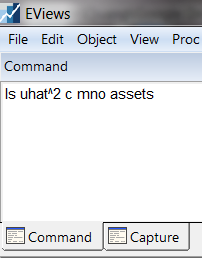
\includegraphics{tute10_1}
\end{figure}
\vspace{-\baselineskip}
%%%%%%%%%% TABLE OBJECT %%%%%%%%%%
\begin{table}[!htbp]
	\centering
	\begin{tabular}{lrrrr}
		\multicolumn{3}{l}{Dependent Variable: UHAT\textasciicircum 2}&\multicolumn{1}{c}{}&\multicolumn{1}{c}{}\\
		\multicolumn{3}{l}{Method: Least Squares}&\multicolumn{1}{c}{}&\multicolumn{1}{c}{}\\
		\multicolumn{3}{l}{Date: 09/15/18   Time: 18:42}&\multicolumn{1}{c}{}&\multicolumn{1}{c}{}\\
		\multicolumn{2}{l}{Sample: 1 88}&\multicolumn{1}{c}{}&\multicolumn{1}{c}{}&\multicolumn{1}{c}{}\\
		\multicolumn{3}{l}{Included observations: 69}&\multicolumn{1}{c}{}&\multicolumn{1}{c}{}\\
		[4.5pt] \hline \\ [-4.5pt]
		\multicolumn{1}{c}{Variable}&\multicolumn{1}{r}{Coefficient}&\multicolumn{1}{r}{Std. Error}&\multicolumn{1}{r}{t-Statistic}&\multicolumn{1}{r}{Prob.}\\
		[4.5pt] \hline \\ [-4.5pt]
		\multicolumn{1}{c}{C}&\multicolumn{1}{r}{$12.83989$}&\multicolumn{1}{r}{$119.7623$}&\multicolumn{1}{r}{$0.107211$}&\multicolumn{1}{r}{$0.9149$}\\
		\multicolumn{1}{c}{MNO}&\multicolumn{1}{r}{$-157.4662$}&\multicolumn{1}{r}{$150.7769$}&\multicolumn{1}{r}{$-1.044365$}&\multicolumn{1}{r}{$0.3001$}\\
		\multicolumn{1}{c}{ASSETS}&\multicolumn{1}{r}{$0.806402$}&\multicolumn{1}{r}{$0.219029$}&\multicolumn{1}{r}{$3.681709$}&\multicolumn{1}{r}{$0.0005$}\\
		[4.5pt] \hline \\ [-4.5pt]
		\multicolumn{1}{l}{R-squared}&\multicolumn{1}{r}{$0.182682$}&\multicolumn{2}{l}{Mean dependent var}&\multicolumn{1}{r}{$163.3550$}\\
		\multicolumn{1}{l}{Adjusted R-squared}&\multicolumn{1}{r}{$0.157914$}&\multicolumn{2}{l}{S.D. dependent var}&\multicolumn{1}{r}{$680.5634$}\\
		\multicolumn{1}{l}{S.E. of regression}&\multicolumn{1}{r}{$624.5205$}&\multicolumn{2}{l}{Akaike info criterion}&\multicolumn{1}{r}{$15.75435$}\\
		\multicolumn{1}{l}{Sum squared resid}&\multicolumn{1}{r}{$25741705$}&\multicolumn{2}{l}{Schwarz criterion}&\multicolumn{1}{r}{$15.85149$}\\
		\multicolumn{1}{l}{Log likelihood}&\multicolumn{1}{r}{$-540.5251$}&\multicolumn{2}{l}{Hannan-Quinn criter.}&\multicolumn{1}{r}{$15.79289$}\\
		\multicolumn{1}{l}{F-statistic}&\multicolumn{1}{r}{$7.375942$}&\multicolumn{2}{l}{Durbin-Watson stat}&\multicolumn{1}{r}{$2.564701$}\\
		\multicolumn{1}{l}{Prob(F-statistic)}&\multicolumn{1}{r}{$0.001285$}&\multicolumn{1}{c}{}&\multicolumn{1}{c}{}&\multicolumn{1}{c}{}\\
		[4.5pt] \hline \\ [-4.5pt]
	\end{tabular}
	%\caption{Add your caption here.}
	%\label{tab:}
\end{table} \vspace{-\baselineskip}\noindent
The estimated auxiliary regression: $$\widehat{\hat{u}^2_i} = 12.8399 - 157.4662 mno_i + 0.8064 assets_i \quad R^2_{aux} = 0.1827$$ The calculated BP test statistic:
$$BP_{calc} = $$

\noindent To obtain the critical value in EViews,
\begin{figure}[H]
	\centering
	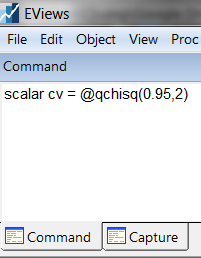
\includegraphics{tute10_2}
\end{figure}
\vspace{-\baselineskip}
\begin{figure}[H]
	\centering
	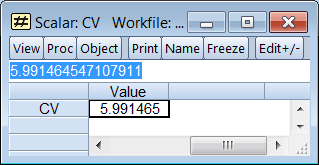
\includegraphics{tute10_3}
\end{figure}
\vspace{-\baselineskip}

\noindent Since $BP_{calc} = 12.6050 > \chi^2_{crit} = 5.99$, 

\noindent Note: EViews has an inbuilt Breusch-Pagan and White test for heteroskedasticity which you can use to verify your results,
$$After\ you\ estimate\ your\ model\ with\ OLS$$
$$From\ the\ equation\ object:$$
$$View \to Residual\ Diagnostics \to Heteroskedasticity\ Tests... $$
\begin{figure}[H]
	\centering
	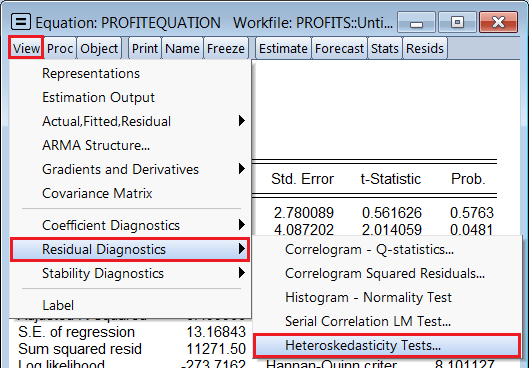
\includegraphics{tute10_6}
\end{figure}
\vspace{-\baselineskip}
\begin{figure}[H]
	\centering
	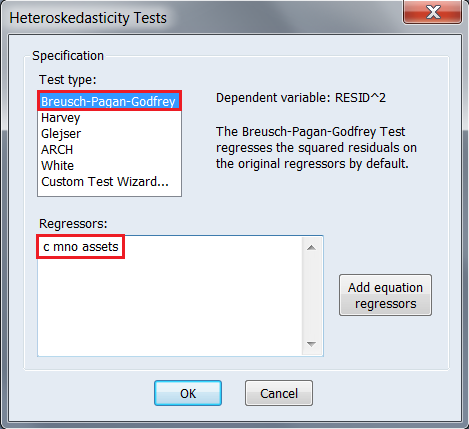
\includegraphics{q1_8}
\end{figure}
\vspace{-\baselineskip}
$$\textbf{Test}\ \textbf{type}: Breusch-Pagan-Godfrey$$ $$\textbf{Regressors}: c \quad mno \quad assets$$
%%%%%%%%%% TABLE OBJECT %%%%%%%%%%
\begin{table}[H]
	\centering
	\begin{tabular}{lrrrr}
		\multicolumn{5}{l}{Heteroskedasticity Test: Breusch-Pagan-Godfrey}\\
		[4.5pt] \hline \\ [-4.5pt]
		\multicolumn{1}{l}{F-statistic}&\multicolumn{1}{r}{$7.375942$}&\multicolumn{2}{l}{Prob. F(2,66)}&\multicolumn{1}{r}{$0.0013$}\\
		\multicolumn{1}{l}{Obs*R-squared}&\multicolumn{1}{r}{$12.60503$}&\multicolumn{2}{l}{Prob. Chi-Square(2)}&\multicolumn{1}{r}{$0.0018$}\\
		\multicolumn{1}{l}{Scaled explained SS}&\multicolumn{1}{r}{$95.66969$}&\multicolumn{2}{l}{Prob. Chi-Square(2)}&\multicolumn{1}{r}{$0.0000$}\\
		[4.5pt] \hline \\ [-4.5pt]
		\multicolumn{1}{c}{}&\multicolumn{1}{c}{}&\multicolumn{1}{c}{}&\multicolumn{1}{c}{}&\multicolumn{1}{c}{}\\
		\multicolumn{2}{l}{Test Equation:}&\multicolumn{1}{c}{}&\multicolumn{1}{c}{}&\multicolumn{1}{c}{}\\
		\multicolumn{3}{l}{Dependent Variable: RESID\textasciicircum 2}&\multicolumn{1}{c}{}&\multicolumn{1}{c}{}\\
		\multicolumn{3}{l}{Method: Least Squares}&\multicolumn{1}{c}{}&\multicolumn{1}{c}{}\\
		\multicolumn{3}{l}{Date: 09/15/18   Time: 19:06}&\multicolumn{1}{c}{}&\multicolumn{1}{c}{}\\
		\multicolumn{2}{l}{Sample: 1 88}&\multicolumn{1}{c}{}&\multicolumn{1}{c}{}&\multicolumn{1}{c}{}\\
		\multicolumn{3}{l}{Included observations: 69}&\multicolumn{1}{c}{}&\multicolumn{1}{c}{}\\
		[4.5pt] \hline \\ [-4.5pt]
		\multicolumn{1}{c}{Variable}&\multicolumn{1}{r}{Coefficient}&\multicolumn{1}{r}{Std. Error}&\multicolumn{1}{r}{t-Statistic}&\multicolumn{1}{r}{Prob.}\\
		[4.5pt] \hline \\ [-4.5pt]
		\multicolumn{1}{c}{C}&\multicolumn{1}{r}{$12.83989$}&\multicolumn{1}{r}{$119.7623$}&\multicolumn{1}{r}{$0.107211$}&\multicolumn{1}{r}{$0.9149$}\\
		\multicolumn{1}{c}{MNO}&\multicolumn{1}{r}{$-157.4662$}&\multicolumn{1}{r}{$150.7769$}&\multicolumn{1}{r}{$-1.044365$}&\multicolumn{1}{r}{$0.3001$}\\
		\multicolumn{1}{c}{ASSETS}&\multicolumn{1}{r}{$0.806402$}&\multicolumn{1}{r}{$0.219029$}&\multicolumn{1}{r}{$3.681709$}&\multicolumn{1}{r}{$0.0005$}\\
		[4.5pt] \hline \\ [-4.5pt]
		\multicolumn{1}{l}{R-squared}&\multicolumn{1}{r}{$0.182682$}&\multicolumn{2}{l}{Mean dependent var}&\multicolumn{1}{r}{$163.3550$}\\
		\multicolumn{1}{l}{Adjusted R-squared}&\multicolumn{1}{r}{$0.157914$}&\multicolumn{2}{l}{S.D. dependent var}&\multicolumn{1}{r}{$680.5634$}\\
		\multicolumn{1}{l}{S.E. of regression}&\multicolumn{1}{r}{$624.5205$}&\multicolumn{2}{l}{Akaike info criterion}&\multicolumn{1}{r}{$15.75435$}\\
		\multicolumn{1}{l}{Sum squared resid}&\multicolumn{1}{r}{$25741705$}&\multicolumn{2}{l}{Schwarz criterion}&\multicolumn{1}{r}{$15.85149$}\\
		\multicolumn{1}{l}{Log likelihood}&\multicolumn{1}{r}{$-540.5251$}&\multicolumn{2}{l}{Hannan-Quinn criter.}&\multicolumn{1}{r}{$15.79289$}\\
		\multicolumn{1}{l}{F-statistic}&\multicolumn{1}{r}{$7.375942$}&\multicolumn{2}{l}{Durbin-Watson stat}&\multicolumn{1}{r}{$2.564701$}\\
		\multicolumn{1}{l}{Prob(F-statistic)}&\multicolumn{1}{r}{$0.001285$}&\multicolumn{1}{c}{}&\multicolumn{1}{c}{}&\multicolumn{1}{c}{}\\
		[4.5pt] \hline \\ [-4.5pt]
	\end{tabular}
	%\caption{Add your caption here.}
	%\label{tab:}
\end{table}
 
\centering
$BP_{calc} = 12.6050 \qquad p-value=0.0018$

\newpage
\justify
\noindent \textcolor{red}{White test}
\justify
\begin{blueframed}
	\textcolor{blue}{\textbf{Background}}
	\vspace{-\baselineskip}
	\justify
	\textcolor{blue}{\underline{White test for heteroskedasticity}}
	
	\noindent \textcolor{blue}
	{
		\noindent If we wish to test for heteroskedasticity without precise knowledge of the relevant variables, we could implement the White test. White's test for heteroskedasticity specifies that the variance of the error term is a function of \textit{all regressors in the model of $y$, the squares of the regressors, and all cross-product combinations of the regressors} (obviously omitting any duplicate variables as this results in perfect collinearity). \\ \\ Our model of $profits$ $$profits_i = \beta_0 + \delta_0 mno_i + \beta_1 assets_i + \delta_1 mno_i^*assets_i + u_i$$ contains the following regressors: \begin{itemize} \vspace{-\baselineskip} \item $mno$
				\item $assets$
				\item $mno^*assets$
			\end{itemize} so the functional form of the error variance for White's test of heteroskedasticity is given by:  \begin{align*}
				Var(u_i|mno_i,assets_i) &= \alpha_0 + \alpha_1 mno_i + \alpha_2 assets_i + \alpha_3 mno_i ^* assets_i + \alpha_4 assets_i^2 \\
				&+ \alpha_5 mno_i^*assets_i^*assets_i
			\end{align*} As you can see, there are no duplicate variables in the error variance e.g. $mno_i$ and $mno_i^2$ are the same variables so only need to include one of them (here I have included $mno_i$ and omitted $mno_i^2$). \\ \\
			Ideally, we would estimate the regression model, \begin{align*}
			u^2_i &= \alpha_0 + \alpha_1 mno_i + \alpha_2 assets_i + \alpha_3 mno_i ^* assets_i + \alpha_4 assets_i^2 \\
			&+ \alpha_5 mno_i^*assets_i^*assets_i + v_i \\
			&= E(u^2_i|mno_i,assets_i) + v_i \\
			&= Var(u_i|mno_i,assets_i) + v_i
			\end{align*} then test if at least one of the variables helps to explain the error variance but this is not feasible because $u^2$ is unobserved. 
	}
\end{blueframed}
\begin{blueframed}
	\vspace{-\baselineskip}
	\justify
	\noindent \textcolor{blue}
	{	To perform's White's test, we replace $u$ with the observed OLS residuals $\hat{u}$ to give us the following \textit{auxiliary regression}: $$\hat{u}^2_i = $$ then test the null and alternative hypothesis: \begin{align*}
		&H_0: E(u^2_i|mno_i,assets_i) =  \\
		&H_1: E(u^2_i|mno_i,assets_i) \neq 
		\end{align*} (The alternative hypothesis is that the variance is a smooth unknown function of $mno_i$ and $assets_i$. $\sigma^2$ and $\delta_0$ are constants. Notation is arbitrary so we could have used $\delta_0$ in our null and alternative hypothesis.) \\ \\
		The White test statistic:
		$$W = $$ $$R^2_{aux}: $$ $$q:$$
	}
\end{blueframed}

\noindent Estimate the auxiliary regression for White's test in EViews,
\begin{figure}[H]
	\centering
	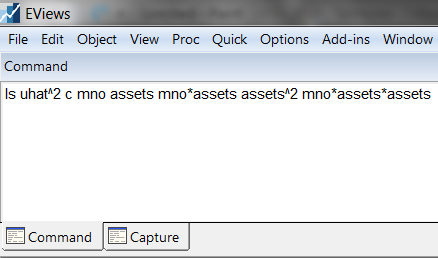
\includegraphics{tute9_3}
\end{figure}
\vspace{-\baselineskip}
%%%%%%%%%% TABLE OBJECT %%%%%%%%%%
\begin{table}[H]
	\centering
	\begin{tabular}{lrrrr}
		\multicolumn{3}{l}{Dependent Variable: UHAT\textasciicircum 2}&\multicolumn{1}{c}{}&\multicolumn{1}{c}{}\\
		\multicolumn{3}{l}{Method: Least Squares}&\multicolumn{1}{c}{}&\multicolumn{1}{c}{}\\
		\multicolumn{3}{l}{Date: 09/16/18   Time: 13:57}&\multicolumn{1}{c}{}&\multicolumn{1}{c}{}\\
		\multicolumn{2}{l}{Sample: 1 88}&\multicolumn{1}{c}{}&\multicolumn{1}{c}{}&\multicolumn{1}{c}{}\\
		\multicolumn{3}{l}{Included observations: 69}&\multicolumn{1}{c}{}&\multicolumn{1}{c}{}\\
		[4.5pt] \hline \\ [-4.5pt]
		\multicolumn{1}{c}{Variable}&\multicolumn{1}{r}{Coefficient}&\multicolumn{1}{r}{Std. Error}&\multicolumn{1}{r}{t-Statistic}&\multicolumn{1}{r}{Prob.}\\
		[4.5pt] \hline \\ [-4.5pt]
		\multicolumn{1}{c}{C}&\multicolumn{1}{r}{$-470.1101$}&\multicolumn{1}{r}{$170.4323$}&\multicolumn{1}{r}{$-2.758340$}&\multicolumn{1}{r}{$0.0076$}\\
		\multicolumn{1}{c}{MNO}&\multicolumn{1}{r}{$536.1701$}&\multicolumn{1}{r}{$263.3993$}&\multicolumn{1}{r}{$2.035579$}&\multicolumn{1}{r}{$0.0460$}\\
		\multicolumn{1}{c}{ASSETS}&\multicolumn{1}{r}{$3.330239$}&\multicolumn{1}{r}{$0.803775$}&\multicolumn{1}{r}{$4.143251$}&\multicolumn{1}{r}{$0.0001$}\\
		\multicolumn{1}{c}{MNO*ASSETS}&\multicolumn{1}{r}{$-3.291956$}&\multicolumn{1}{r}{$1.244107$}&\multicolumn{1}{r}{$-2.646040$}&\multicolumn{1}{r}{$0.0103$}\\
		\multicolumn{1}{c}{ASSETS\textasciicircum 2}&\multicolumn{1}{r}{$-0.001130$}&\multicolumn{1}{r}{$0.000452$}&\multicolumn{1}{r}{$-2.498314$}&\multicolumn{1}{r}{$0.0151$}\\
		\multicolumn{1}{c}{MNO*ASSETS*ASSETS}&\multicolumn{1}{r}{$0.001122$}&\multicolumn{1}{r}{$0.000663$}&\multicolumn{1}{r}{$1.692514$}&\multicolumn{1}{r}{$0.0955$}\\
		[4.5pt] \hline \\ [-4.5pt]
		\multicolumn{1}{l}{R-squared}&\multicolumn{1}{r}{$0.371760$}&\multicolumn{2}{l}{Mean dependent var}&\multicolumn{1}{r}{$163.3550$}\\
		\multicolumn{1}{l}{Adjusted R-squared}&\multicolumn{1}{r}{$0.321900$}&\multicolumn{2}{l}{S.D. dependent var}&\multicolumn{1}{r}{$680.5634$}\\
		\multicolumn{1}{l}{S.E. of regression}&\multicolumn{1}{r}{$560.4225$}&\multicolumn{2}{l}{Akaike info criterion}&\multicolumn{1}{r}{$15.57820$}\\
		\multicolumn{1}{l}{Sum squared resid}&\multicolumn{1}{r}{$19786623$}&\multicolumn{2}{l}{Schwarz criterion}&\multicolumn{1}{r}{$15.77247$}\\
		\multicolumn{1}{l}{Log likelihood}&\multicolumn{1}{r}{$-531.4479$}&\multicolumn{2}{l}{Hannan-Quinn criter.}&\multicolumn{1}{r}{$15.65527$}\\
		\multicolumn{1}{l}{F-statistic}&\multicolumn{1}{r}{$7.456027$}&\multicolumn{2}{l}{Durbin-Watson stat}&\multicolumn{1}{r}{$2.531454$}\\
		\multicolumn{1}{l}{Prob(F-statistic)}&\multicolumn{1}{r}{$0.000015$}&\multicolumn{1}{c}{}&\multicolumn{1}{c}{}&\multicolumn{1}{c}{}\\
		[4.5pt] \hline \\ [-4.5pt]
	\end{tabular}
	%\caption{Add your caption here.}
	%\label{tab:}
\end{table}
\vspace{-\baselineskip} \noindent The estimated auxiliary regression:
\begin{align*}
	\widehat{\hat{u}^2_i} =
\end{align*}
$$R^2_{aux} = 0.3718$$ The calculated White test statistics:
$$W_{calc} = $$ \noindent To obtain the critical value in EViews,
\begin{figure}[H]
	\centering
	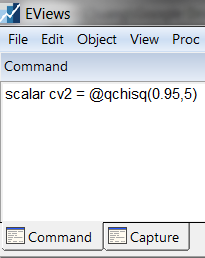
\includegraphics{tute9_4}
\end{figure}
\vspace{-\baselineskip}
\begin{figure}[H]
	\centering
	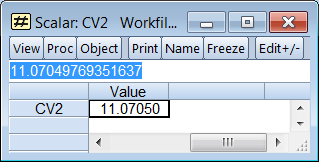
\includegraphics{tute9_5}
\end{figure}
\vspace{-\baselineskip}

\noindent Since $W_{calc} = 25.6542 > W_{crit} = 11.0705$, we reject $H_0$ at the 5\% significance level and conclude that there is sufficient evidence from our sample to suggest that the errors are heteroskedastic.



\noindent Using the in-built White test in EViews:
$$After\ you\ estimate\ your\ model\ with\ OLS$$
$$From\ the\ equation\ object:$$
$$View \to Residual\ Diagnostics \to Heteroskedasticity\ Tests... $$
\begin{figure}[H]
	\centering
	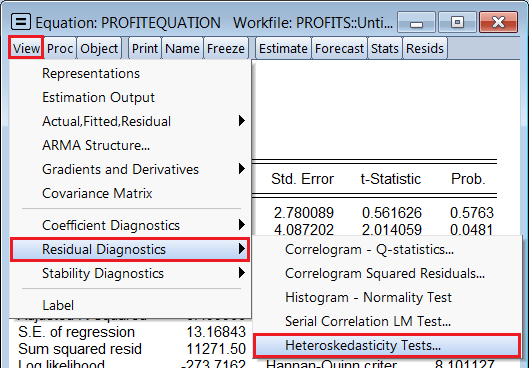
\includegraphics{tute10_6}
\end{figure}
\vspace{-\baselineskip}
\begin{figure}[H]
	\centering
	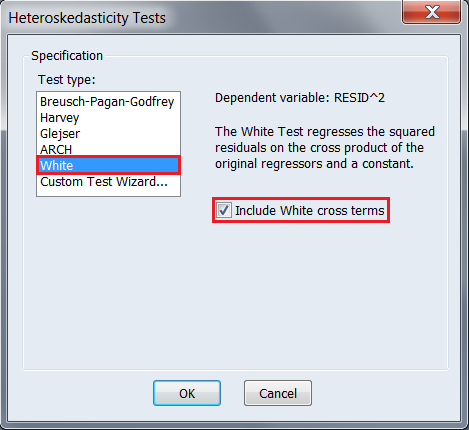
\includegraphics{tute9_2}
\end{figure}
\vspace{-\baselineskip}
$$\textbf{Test}\ \textbf{type}: White$$
%%%%%%%%%% TABLE OBJECT %%%%%%%%%%
\begin{table}[H]
	\centering
	\begin{tabular}{lrrrr}
		\multicolumn{3}{l}{Heteroskedasticity Test: White}&\multicolumn{1}{c}{}&\multicolumn{1}{c}{}\\
		[4.5pt] \hline \\ [-4.5pt]
		\multicolumn{1}{l}{F-statistic}&\multicolumn{1}{r}{$7.456027$}&\multicolumn{2}{l}{Prob. F(5,63)}&\multicolumn{1}{r}{$0.0000$}\\
		\multicolumn{1}{l}{Obs*R-squared}&\multicolumn{1}{r}{$25.65143$}&\multicolumn{2}{l}{Prob. Chi-Square(5)}&\multicolumn{1}{r}{$0.0001$}\\
		\multicolumn{1}{l}{Scaled explained SS}&\multicolumn{1}{r}{$194.6893$}&\multicolumn{2}{l}{Prob. Chi-Square(5)}&\multicolumn{1}{r}{$0.0000$}\\
		[4.5pt] \hline \\ [-4.5pt]
		\multicolumn{1}{c}{}&\multicolumn{1}{c}{}&\multicolumn{1}{c}{}&\multicolumn{1}{c}{}&\multicolumn{1}{c}{}\\
		\multicolumn{2}{l}{Test Equation:}&\multicolumn{1}{c}{}&\multicolumn{1}{c}{}&\multicolumn{1}{c}{}\\
		\multicolumn{3}{l}{Dependent Variable: RESID\textasciicircum 2}&\multicolumn{1}{c}{}&\multicolumn{1}{c}{}\\
		\multicolumn{3}{l}{Method: Least Squares}&\multicolumn{1}{c}{}&\multicolumn{1}{c}{}\\
		\multicolumn{3}{l}{Date: 09/16/18   Time: 09:08}&\multicolumn{1}{c}{}&\multicolumn{1}{c}{}\\
		\multicolumn{2}{l}{Sample: 1 88}&\multicolumn{1}{c}{}&\multicolumn{1}{c}{}&\multicolumn{1}{c}{}\\
		\multicolumn{3}{l}{Included observations: 69}&\multicolumn{1}{c}{}&\multicolumn{1}{c}{}\\
		\multicolumn{5}{l}{Collinear test regressors dropped from specification}\\
		[4.5pt] \hline \\ [-4.5pt]
		\multicolumn{1}{c}{Variable}&\multicolumn{1}{r}{Coefficient}&\multicolumn{1}{r}{Std. Error}&\multicolumn{1}{r}{t-Statistic}&\multicolumn{1}{r}{Prob.}\\
		[4.5pt] \hline \\ [-4.5pt]
		\multicolumn{1}{c}{C}&\multicolumn{1}{r}{$-470.1101$}&\multicolumn{1}{r}{$170.4323$}&\multicolumn{1}{r}{$-2.758340$}&\multicolumn{1}{r}{$0.0076$}\\
		\multicolumn{1}{c}{MNO\textasciicircum 2}&\multicolumn{1}{r}{$536.1701$}&\multicolumn{1}{r}{$263.3993$}&\multicolumn{1}{r}{$2.035579$}&\multicolumn{1}{r}{$0.0460$}\\
		\multicolumn{1}{c}{MNO*ASSETS}&\multicolumn{1}{r}{$-3.291956$}&\multicolumn{1}{r}{$1.244107$}&\multicolumn{1}{r}{$-2.646040$}&\multicolumn{1}{r}{$0.0103$}\\
		\multicolumn{1}{c}{ASSETS\textasciicircum 2}&\multicolumn{1}{r}{$-0.001130$}&\multicolumn{1}{r}{$0.000452$}&\multicolumn{1}{r}{$-2.498314$}&\multicolumn{1}{r}{$0.0151$}\\
		\multicolumn{1}{c}{ASSETS*MNO*ASSETS}&\multicolumn{1}{r}{$0.001122$}&\multicolumn{1}{r}{$0.000663$}&\multicolumn{1}{r}{$1.692514$}&\multicolumn{1}{r}{$0.0955$}\\
		\multicolumn{1}{c}{ASSETS}&\multicolumn{1}{r}{$3.330239$}&\multicolumn{1}{r}{$0.803775$}&\multicolumn{1}{r}{$4.143251$}&\multicolumn{1}{r}{$0.0001$}\\
		[4.5pt] \hline \\ [-4.5pt]
		\multicolumn{1}{l}{R-squared}&\multicolumn{1}{r}{$0.371760$}&\multicolumn{2}{l}{Mean dependent var}&\multicolumn{1}{r}{$163.3550$}\\
		\multicolumn{1}{l}{Adjusted R-squared}&\multicolumn{1}{r}{$0.321900$}&\multicolumn{2}{l}{S.D. dependent var}&\multicolumn{1}{r}{$680.5634$}\\
		\multicolumn{1}{l}{S.E. of regression}&\multicolumn{1}{r}{$560.4225$}&\multicolumn{2}{l}{Akaike info criterion}&\multicolumn{1}{r}{$15.57820$}\\
		\multicolumn{1}{l}{Sum squared resid}&\multicolumn{1}{r}{$19786623$}&\multicolumn{2}{l}{Schwarz criterion}&\multicolumn{1}{r}{$15.77247$}\\
		\multicolumn{1}{l}{Log likelihood}&\multicolumn{1}{r}{$-531.4479$}&\multicolumn{2}{l}{Hannan-Quinn criter.}&\multicolumn{1}{r}{$15.65527$}\\
		\multicolumn{1}{l}{F-statistic}&\multicolumn{1}{r}{$7.456027$}&\multicolumn{2}{l}{Durbin-Watson stat}&\multicolumn{1}{r}{$2.531454$}\\
		\multicolumn{1}{l}{Prob(F-statistic)}&\multicolumn{1}{r}{$0.000015$}&\multicolumn{1}{c}{}&\multicolumn{1}{c}{}&\multicolumn{1}{c}{}\\
		[4.5pt] \hline \\ [-4.5pt]
	\end{tabular}
	%\caption{Add your caption here.}
	%\label{tab:}
\end{table}


\noindent \textcolor{red}{Special form of the White test that uses the predicted value of $profits$ and its square as predictors of variance.} 
\begin{align*}
	H_0&: Var(u_i|mno_i,assets_i) = \sigma^2 \\
	H_1&: Var(u_i|mno_i,assets_i) \neq \sigma^2
\end{align*} The alternative hypothesis is that the error variance is a smooth unknown function of $mno_i$ and $assets_i$.

\noindent The functional form of the error variance for this special form of White test: $$Var(u_i|mno_i,assets_i) = $$

\noindent The auxiliary regression: $$\hat{u}^2_i = $$

\noindent Before estimating the auxiliary regression, we should save $\widehat{profit}_i$ as a variable in our EViews workfile. From the Command Window: $$genr\ profithat = profits-uhat$$
\begin{figure}[H]
	\centering
	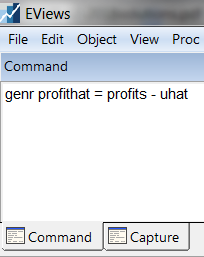
\includegraphics{tute9_6}
\end{figure}
\vspace{-\baselineskip} \noindent This generates a new object called $profithat$ which is equal to $profits$ minus the OLS residual $uhat$. Note, $uhat$ is the OLS residual (from the estimated model of $profits$) that we saved earlier.
\begin{figure}[H]
	\centering
	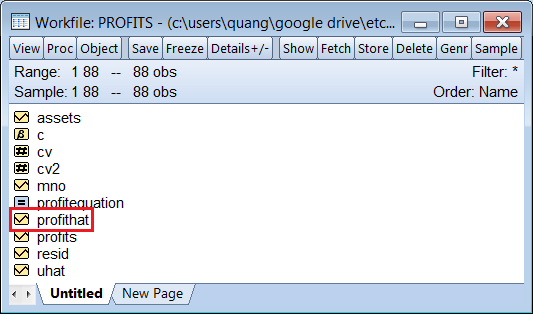
\includegraphics{tute9_7}
\end{figure}
\vspace{-\baselineskip} \noindent To estimate the auxiliary regression from the Command Window in EViews: $$ls\ uhat^2\ c\ profitshat\ profitshat^2$$
\begin{figure}[H]
	\centering
	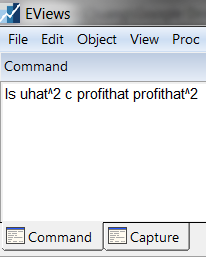
\includegraphics{tute9_8}
\end{figure}
\vspace{-\baselineskip}

%%%%%%%%%% TABLE OBJECT %%%%%%%%%%
\begin{table}[H]
	\centering
	\begin{tabular}{lrrrr}
		\multicolumn{3}{l}{Dependent Variable: UHAT\textasciicircum 2}&\multicolumn{1}{c}{}&\multicolumn{1}{c}{}\\
		\multicolumn{3}{l}{Method: Least Squares}&\multicolumn{1}{c}{}&\multicolumn{1}{c}{}\\
		\multicolumn{3}{l}{Date: 09/16/18   Time: 17:54}&\multicolumn{1}{c}{}&\multicolumn{1}{c}{}\\
		\multicolumn{2}{l}{Sample: 1 88}&\multicolumn{1}{c}{}&\multicolumn{1}{c}{}&\multicolumn{1}{c}{}\\
		\multicolumn{3}{l}{Included observations: 69}&\multicolumn{1}{c}{}&\multicolumn{1}{c}{}\\
		[4.5pt] \hline \\ [-4.5pt]
		\multicolumn{1}{c}{Variable}&\multicolumn{1}{r}{Coefficient}&\multicolumn{1}{r}{Std. Error}&\multicolumn{1}{r}{t-Statistic}&\multicolumn{1}{r}{Prob.}\\
		[4.5pt] \hline \\ [-4.5pt]
		\multicolumn{1}{c}{C}&\multicolumn{1}{r}{$-529.7017$}&\multicolumn{1}{r}{$161.4841$}&\multicolumn{1}{r}{$-3.280210$}&\multicolumn{1}{r}{$0.0017$}\\
		\multicolumn{1}{c}{PROFITHAT}&\multicolumn{1}{r}{$65.44824$}&\multicolumn{1}{r}{$15.73677$}&\multicolumn{1}{r}{$4.158937$}&\multicolumn{1}{r}{$0.0001$}\\
		\multicolumn{1}{c}{PROFITHAT\textasciicircum 2}&\multicolumn{1}{r}{$-0.427865$}&\multicolumn{1}{r}{$0.171206$}&\multicolumn{1}{r}{$-2.499129$}&\multicolumn{1}{r}{$0.0149$}\\
		[4.5pt] \hline \\ [-4.5pt]
		\multicolumn{1}{l}{R-squared}&\multicolumn{1}{r}{$0.368618$}&\multicolumn{2}{l}{Mean dependent var}&\multicolumn{1}{r}{$163.3550$}\\
		\multicolumn{1}{l}{Adjusted R-squared}&\multicolumn{1}{r}{$0.349485$}&\multicolumn{2}{l}{S.D. dependent var}&\multicolumn{1}{r}{$680.5634$}\\
		\multicolumn{1}{l}{S.E. of regression}&\multicolumn{1}{r}{$548.9051$}&\multicolumn{2}{l}{Akaike info criterion}&\multicolumn{1}{r}{$15.49623$}\\
		\multicolumn{1}{l}{Sum squared resid}&\multicolumn{1}{r}{$19885591$}&\multicolumn{2}{l}{Schwarz criterion}&\multicolumn{1}{r}{$15.59337$}\\
		\multicolumn{1}{l}{Log likelihood}&\multicolumn{1}{r}{$-531.6200$}&\multicolumn{2}{l}{Hannan-Quinn criter.}&\multicolumn{1}{r}{$15.53477$}\\
		\multicolumn{1}{l}{F-statistic}&\multicolumn{1}{r}{$19.26627$}&\multicolumn{2}{l}{Durbin-Watson stat}&\multicolumn{1}{r}{$2.541133$}\\
		\multicolumn{1}{l}{Prob(F-statistic)}&\multicolumn{1}{r}{$0.000000$}&\multicolumn{1}{c}{}&\multicolumn{1}{c}{}&\multicolumn{1}{c}{}\\
		[4.5pt] \hline \\ [-4.5pt]
	\end{tabular}
	%\caption{Add your caption here.}
	%\label{tab:}
\end{table} \vspace{-\baselineskip} \noindent
The White test statistic:
$$W = n \times R^2_{aux} \sim \chi_{q=2}^2 \quad under\ H_0$$ $$R^2_{aux}: R^2\ from\ the\ auxiliary\ regression$$ $$q:number\ of\ regressors\ in\ the\ auxiliary\ regression$$ The calculated White test statistic: $$W_{calc} = 69 \times 0.3686 = 25.4334$$ The critical value: $$W_{crit} = \chi^2_{crit} = \chi_{2,0.95}^2 = 5.99$$

\noindent Since $W_{calc} = 25.4334 > W_{crit} = 5.99$, 



\newpage
\justify
\noindent \textcolor{red}
{
	(c) Is it likely that a log-log formulation that uses $log(profits)$ and $log(assets)$ would solve the heteroskedasticity problem in this application? Explain.
}

\noindent \uline{Lec8 - page 21}

\noindent \textit{If the population model has $log(y)$ as the dependent variable but we have used $y$, this kind of mis-specification can show up as heteroskedastic errors. So, if log-transformation is admissible (i.e. if $y$ is positive), moving to a log model may solve the problem, and the OLS estimator on the log-transformed model will then be BLUE and standard errors will be useful. Of course, when we consider transforming $y$, we should think if a log-level or a log-log model makes better sense.}

\noindent Since $profits$ can be negative, log transformation is not an option.


\newpage
\justify
\noindent \textcolor{red}
{
	(d) In each of the following scenarios, determine the appropriate weight that solves the problem of heteroskedasticity when it multiplies on both sides of the equation of $profits$: \begin{align*}
		Var(u_i|mno_i, assets_i) &= \sigma^2 \times assets_i \\
		Var(u_i|mno_i, assets_i) &= \sigma^2 \times assets_i^2 \\
		Var(u_i|mno_i, assets_i) &= \sigma^2 \times log(assets_i)
	\end{align*}
}

\justify
\begin{blueframed}
	\textcolor{blue}{\textbf{Background}}
	\vspace{-\baselineskip}
	\justify
	\textcolor{blue}{\underline{Weighted Least Squares Estimator}}
	
	\noindent \textcolor{blue}
	{
		\noindent It is helpful to consider the WLS estimator as a 2-step estimator: \begin{itemize}
			\item At step 1, apply some weighting/transformation to the original model to obtain the weighted model.
			\item At step 2, estimate the weighted model by OLS.
		\end{itemize} If the variance of the error has the following known functional form,
		$$Var(u_i|x_{i1},x_{i2},...) = \sigma^2 \times h_i$$
		\noindent then weighing the original model by,
		$$w_i = \dfrac{1}{\sqrt{h_i}}$$
		\noindent produces the following weighted model, $$w_iy_i = \beta_0w_i + \beta_1w_ix_{i1} + \beta_2w_ix_{i2} + \dots + w_iu_i$$ with a constant error variance 		(homoskedastic error),
		\begin{align*}
		Var(w_iu_i|x_{i1},x_{i2},\dots) &= w^2_iVar(u_i|x_{i1},x_{i2},\dots) \\
		&= \dfrac{1}{h_i}Var(u_i|x_{i1},x_{i2},\dots) \\
		&= \dfrac{1}{h_i}\sigma^2h_i \\
		&= \sigma^2
		\end{align*}
		The weight, $w_i$, is known and not treated a random variable. \\ \\ The Weighted Least Squares (WLS) estimator is the OLS estimator used to estimate the weighted model of $y$ (weighted so that the error has constant variance).
	}
\end{blueframed}

\noindent If the variance of the error takes the following form,
$$Var(u_i|mno_i, assets_i) = \sigma^2 \times assets_i$$
\noindent then the weight that we need to apply to our original model to obtain a weighted model with constant error variance (homoskedastic error) is given by,
$$w_i = \dfrac{1}{\sqrt{assets_i}}$$
\noindent Multiplying $w_i$ on both sides of the original model of $profits_i$ gives the following weighted model of $profits_i$,
$$\dfrac{profits_i}{\sqrt{assets_i}} = \dfrac{\beta_0}{\sqrt{assets_i}} + \dfrac{\delta_0mno_i}{\sqrt{assets_i}} + \dfrac{\beta_1assets_i}{\sqrt{assets_i}} + \dfrac{\delta_1mno_i^*assets_i}{\sqrt{assets_i}} + \dfrac{u_i}{\sqrt{assets_i}}$$

\noindent and the error term in this weighted model has constant variance,
\begin{align*}
Var(\dfrac{u_i}{\sqrt{assets_i}}|mno_i,assets_i) &= \dfrac{1}{assets_i}Var(u_i|mno_i,assets_i) \\
&= \dfrac{1}{assets_i}\sigma^2 \times assets_i \\
&= \sigma^2
\end{align*}

\noindent If the variance of the error takes the following form,
$$Var(u_i|mno_i, assets_i) = \sigma^2 \times assets_i^2$$
\noindent then the weight that we need to apply to our original model to obtain a weighted model with constant error variance (homoskedastic error) is given by,
$$w_i = \dfrac{1}{assets_i}$$

\noindent If the variance of the error takes the following form,
$$Var(u_i|mno_i, assets_i) = \sigma^2 \times assets_i^2$$
\noindent then the weight that we need to apply to our original model to obtain a weighted model with constant error variance (homoskedastic error) is given by,
$$w_i = \dfrac{1}{log(assets_i)}$$

\newpage
\noindent \textcolor{red}
{
	(e) Suppose we know $Var(u_i|mno_i,assets_i) = \sigma^2 \times assets_i$. Test the hypothesis that you formulated in part (a), i.e. that the nature of the ownership of a firm does not effect the relationship between its profits and its assets against the alternative that it does.
}

\noindent If $Var(u_i|mno_i,assets_i) = \sigma^2 \times assets_i$ then our weighted model of $profits$ is given by: $$\dfrac{profits_i}{\sqrt{assets_i}} = \dfrac{\beta_0}{\sqrt{assets_i}} + \dfrac{\delta_0mno_i}{\sqrt{assets_i}} + \dfrac{\beta_1assets_i}{\sqrt{assets_i}} + \dfrac{\delta_1mno_i^*assets_i}{\sqrt{assets_i}} + \dfrac{u_i}{\sqrt{assets_i}}$$

\noindent We wish to test the null hypothesis the nature of ownership of a firm does not effect the relationship between its profits and assets, $$H_0: \delta_0 = \delta_1 = 0$$ against the alternative hypothesis that it does, $$H_1:\delta_0 \neq 0\ and/or\ \delta_1 \neq 0$$ Since we are testing multiple linear restrictions (2 restrictions), we require a F test. $$F = \dfrac{(SSR_r - SSR_{ur})/q}{SSR_{ur}/(n-k-1)} = \dfrac{(SSR_r - SSR_{ur})/2}{SSR_{ur}/(69-3-1)} \sim F_{2,65} \quad under\ H_0$$
\begin{align*}
n &= sample\ size = 69 \\
k &= number\ of\ regressors\ in\ the\ unrestricted\ model = 3 \\
q &= number\ of\ restrictions\ = 2 \\
SSR_{r} &= sum\ of\ squared\ residuals\ from\ estimated\ restricted\ model \\
SSR_{ur} &= sum\ of\ squared\ residuals\ from\ estimated\ unrestricted\ model
\end{align*}

\noindent The unrestricted and restricted model:

\noindent Before estimating the unrestricted and restricted, let us generate the variable $w = \dfrac{1}{\sqrt{assets}}$ in EViews. From the Command Window: $$genr\ w=1/@sqrt(assets)$$
\begin{figure}[H]
	\centering
	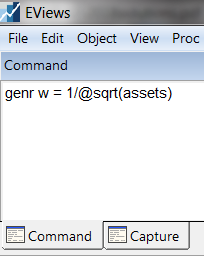
\includegraphics{tute9_9}
\end{figure}
\vspace{-\baselineskip}
\begin{figure}[H]
	\centering
	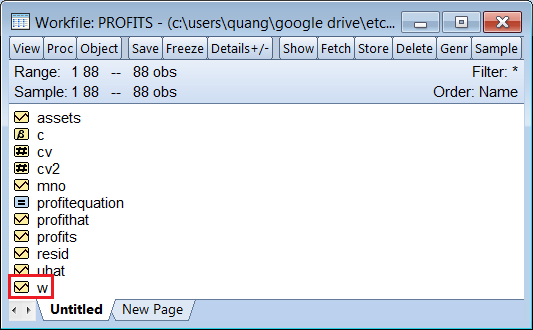
\includegraphics{tute9_10}
\end{figure}
\vspace{-\baselineskip}

\noindent To estimate the weighted unrestricted model from the Command Window,
$$ls\ w\ w^*mno\ w^*assets\ w^*mno^*assets$$
\begin{figure}[H]
	\centering
	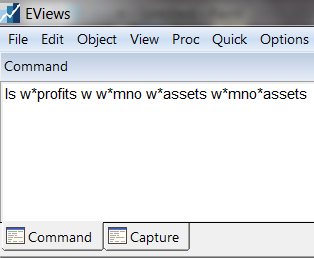
\includegraphics{tute9_11}
\end{figure}
\vspace{-\baselineskip}
%%%%%%%%%% TABLE OBJECT %%%%%%%%%%
\begin{table}[H]
	\centering
	\begin{tabular}{lrrrr}
		\multicolumn{4}{l}{Dependent Variable: W*PROFITS}&\multicolumn{1}{c}{}\\
		\multicolumn{3}{l}{Method: Least Squares}&\multicolumn{1}{c}{}&\multicolumn{1}{c}{}\\
		\multicolumn{3}{l}{Date: 09/17/18   Time: 19:47}&\multicolumn{1}{c}{}&\multicolumn{1}{c}{}\\
		\multicolumn{2}{l}{Sample: 1 88}&\multicolumn{1}{c}{}&\multicolumn{1}{c}{}&\multicolumn{1}{c}{}\\
		\multicolumn{3}{l}{Included observations: 69}&\multicolumn{1}{c}{}&\multicolumn{1}{c}{}\\
		[4.5pt] \hline \\ [-4.5pt]
		\multicolumn{1}{c}{Variable}&\multicolumn{1}{r}{Coefficient}&\multicolumn{1}{r}{Std. Error}&\multicolumn{1}{r}{t-Statistic}&\multicolumn{1}{r}{Prob.}\\
		[4.5pt] \hline \\ [-4.5pt]
		\multicolumn{1}{c}{W}&\multicolumn{1}{r}{$0.123099$}&\multicolumn{1}{r}{$1.937385$}&\multicolumn{1}{r}{$0.063539$}&\multicolumn{1}{r}{$0.9495$}\\
		\multicolumn{1}{c}{W*MNO}&\multicolumn{1}{r}{$2.500248$}&\multicolumn{1}{r}{$2.657450$}&\multicolumn{1}{r}{$0.940845$}&\multicolumn{1}{r}{$0.3503$}\\
		\multicolumn{1}{c}{W*ASSETS}&\multicolumn{1}{r}{$0.055756$}&\multicolumn{1}{r}{$0.009207$}&\multicolumn{1}{r}{$6.056060$}&\multicolumn{1}{r}{$0.0000$}\\
		\multicolumn{1}{c}{W*MNO*ASSETS}&\multicolumn{1}{r}{$-0.030944$}&\multicolumn{1}{r}{$0.013195$}&\multicolumn{1}{r}{$-2.345092$}&\multicolumn{1}{r}{$0.0221$}\\
		[4.5pt] \hline \\ [-4.5pt]
		\multicolumn{1}{l}{R-squared}&\multicolumn{1}{r}{$0.175888$}&\multicolumn{2}{l}{Mean dependent var}&\multicolumn{1}{r}{$0.748290$}\\
		\multicolumn{1}{l}{Adjusted R-squared}&\multicolumn{1}{r}{$0.137852$}&\multicolumn{2}{l}{S.D. dependent var}&\multicolumn{1}{r}{$0.672177$}\\
		\multicolumn{1}{l}{S.E. of regression}&\multicolumn{1}{r}{$0.624129$}&\multicolumn{2}{l}{Akaike info criterion}&\multicolumn{1}{r}{$1.951304$}\\
		\multicolumn{1}{l}{Sum squared resid}&\multicolumn{1}{r}{$25.31993$}&\multicolumn{2}{l}{Schwarz criterion}&\multicolumn{1}{r}{$2.080818$}\\
		\multicolumn{1}{l}{Log likelihood}&\multicolumn{1}{r}{$-63.32000$}&\multicolumn{2}{l}{Hannan-Quinn criter.}&\multicolumn{1}{r}{$2.002687$}\\
		\multicolumn{1}{l}{Durbin-Watson stat}&\multicolumn{1}{r}{$2.179079$}&\multicolumn{1}{c}{}&\multicolumn{1}{c}{}&\multicolumn{1}{c}{}\\
		[4.5pt] \hline \\ [-4.5pt]
	\end{tabular}
	%\caption{Add your caption here.}
	%\label{tab:}
\end{table} \vspace{-\baselineskip}
$$\widehat{w^*profits}_i = \underset{(1.9374)}{0.1231}w + \underset{(2.6575)}{2.5002}w^*mno + \underset{(0.0092)}{0.0448}w^*assets - \underset{(0.0131)}{0.0309}w^*mno^*assets$$ $$SSR_{ur} = 25.3199$$
\noindent To estimate the weighted model from the Command Window,
$$ls\ w\ w^*assets$$
\begin{figure}[H]
	\centering
	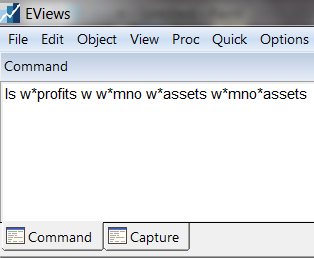
\includegraphics{tute9_11}
\end{figure}
\vspace{-\baselineskip} 


%%%%%%%%%% TABLE OBJECT %%%%%%%%%%
\begin{table}[H]
	\centering
	\begin{tabular}{lrrrr}
		\multicolumn{4}{l}{Dependent Variable: W*PROFITS}&\multicolumn{1}{c}{}\\
		\multicolumn{3}{l}{Method: Least Squares}&\multicolumn{1}{c}{}&\multicolumn{1}{c}{}\\
		\multicolumn{3}{l}{Date: 09/17/18   Time: 19:56}&\multicolumn{1}{c}{}&\multicolumn{1}{c}{}\\
		\multicolumn{2}{l}{Sample: 1 88}&\multicolumn{1}{c}{}&\multicolumn{1}{c}{}&\multicolumn{1}{c}{}\\
		\multicolumn{3}{l}{Included observations: 69}&\multicolumn{1}{c}{}&\multicolumn{1}{c}{}\\
		[4.5pt] \hline \\ [-4.5pt]
		\multicolumn{1}{c}{Variable}&\multicolumn{1}{r}{Coefficient}&\multicolumn{1}{r}{Std. Error}&\multicolumn{1}{r}{t-Statistic}&\multicolumn{1}{r}{Prob.}\\
		[4.5pt] \hline \\ [-4.5pt]
		\multicolumn{1}{c}{W}&\multicolumn{1}{r}{$1.395225$}&\multicolumn{1}{r}{$1.371934$}&\multicolumn{1}{r}{$1.016977$}&\multicolumn{1}{r}{$0.3128$}\\
		\multicolumn{1}{c}{W*ASSETS}&\multicolumn{1}{r}{$0.041256$}&\multicolumn{1}{r}{$0.006804$}&\multicolumn{1}{r}{$6.063294$}&\multicolumn{1}{r}{$0.0000$}\\
		[4.5pt] \hline \\ [-4.5pt]
		\multicolumn{1}{l}{R-squared}&\multicolumn{1}{r}{$0.090491$}&\multicolumn{2}{l}{Mean dependent var}&\multicolumn{1}{r}{$0.748290$}\\
		\multicolumn{1}{l}{Adjusted R-squared}&\multicolumn{1}{r}{$0.076916$}&\multicolumn{2}{l}{S.D. dependent var}&\multicolumn{1}{r}{$0.672177$}\\
		\multicolumn{1}{l}{S.E. of regression}&\multicolumn{1}{r}{$0.645809$}&\multicolumn{2}{l}{Akaike info criterion}&\multicolumn{1}{r}{$1.991932$}\\
		\multicolumn{1}{l}{Sum squared resid}&\multicolumn{1}{r}{$27.94365$}&\multicolumn{2}{l}{Schwarz criterion}&\multicolumn{1}{r}{$2.056688$}\\
		\multicolumn{1}{l}{Log likelihood}&\multicolumn{1}{r}{$-66.72164$}&\multicolumn{2}{l}{Hannan-Quinn criter.}&\multicolumn{1}{r}{$2.017623$}\\
		\multicolumn{1}{l}{Durbin-Watson stat}&\multicolumn{1}{r}{$2.223289$}&\multicolumn{1}{c}{}&\multicolumn{1}{c}{}&\multicolumn{1}{c}{}\\
		[4.5pt] \hline \\ [-4.5pt]
	\end{tabular}
	%\caption{Add your caption here.}
	%\label{tab:}
\end{table}
\vspace{-\baselineskip} $$\widehat{w^*profits}_i = \underset{(1.3719)}{1.3952}w + \underset{(0.0068)}{0.0413}w^*assets$$ $$SSR_r = 27.9437$$

$$F_{calc} = \dfrac{(SSR_r - SSR_{ur})/2}{SSR_{ur}/(65)} = \dfrac{(27.94-25.32)/2}{25.32/(65)} = 3.36$$
$$F_{crit} = 3.15 \quad (5\%\ level.\ Stat\ Table)$$
\noindent Since $F_{calc}=3.36 > F_{crit}=3.15$, we reject the null at the 5\% significance level and conclude that there is some difference in the relationship between profits and assets across owner managed and non-owner managed firms.

\noindent Note: This process of applying a weighted transformation to the model is a device to converting a model with heteroskedastic errors into one with homoskedasticity error. It is NOT something that changes the inherent meaning of the coefficients. As such, we still interpret the ‘weighted’ coefficients the same way as we would with the original model.








\end{document}